\documentclass[11pt]{article}

% some definitions for the title page
\newcommand{\reporttitle}{Causality and Generative Models}
\newcommand{\reportdescription}{}

% load some definitions and default packages
%---------------------------------------------------------------------------
%	PACKAGES AND OTHER DOCUMENT CONFIGURATIONS
%---------------------------------------------------------------------------

\usepackage[twoside]{fancyhdr}
\usepackage{csquotes}

\usepackage[a4paper,hmargin=2.0cm,vmargin=1.0cm,includeheadfoot]{geometry}
% \usepackage{natbib} % for bibliography
\usepackage{biblatex}
\usepackage{tabularx,longtable,multirow,subfigure,caption}%hangcaption
\usepackage{fancyhdr} % page layout
\usepackage{url} % URLs
\usepackage[english]{babel}
\usepackage{graphicx}
\usepackage{rotating}
\usepackage{dsfont}
\usepackage{epstopdf} % automatically replace .eps with .pdf in graphics
% \usepackage{backref} % needed for citations
\usepackage{array}
\usepackage{latexsym}
\usepackage[pdftex,hypertexnames=false,colorlinks]{hyperref} % provide links in pdf (had pagebackref)
\usepackage{booktabs}
\usepackage{wrapfig}
\usepackage{caption}  % Required for \captionof
\usepackage{float} % for H option in figures
\usepackage{amssymb}
\usepackage{amsmath}
\usepackage{amsthm}
\usepackage{mathtools} % for 'dcases*' env.
\usepackage[nottoc]{tocbibind}

%%% Default fonts
\renewcommand*{\rmdefault}{bch}
\renewcommand*{\ttdefault}{cmtt}

%%% Default settings (page layout)
\setlength{\parindent}{0em}  % indentation of paragraph
\setlength{\parskip}{.3em}
\setlength{\itemsep}{0.mm}

\setlength{\headheight}{14.5pt}
\pagestyle{fancy}

\fancyfoot[ER,OL]{\thepage}%Page no. in the left on odd pages and on right on even pages

\fancyfoot[OC,EC]{\sffamily }
\renewcommand{\headrulewidth}{0.1pt}
\renewcommand{\footrulewidth}{0.1pt}
\captionsetup{margin=10pt,font=small,labelfont=bf}

% LISTINGS ammendments
\usepackage{listings}
\usepackage{color}

\definecolor{mygreen}{rgb}{0,0.6,0}
\definecolor{mygray}{rgb}{0.5,0.5,0.5}
\definecolor{mymauve}{rgb}{0.58,0,0.82}

\lstset{ 
  postbreak=\mbox{\textcolor{red}{$\hookrightarrow$}\space},
  backgroundcolor=\color{white},   % choose the background color; you must add \usepackage{color} or \usepackage{xcolor}; should come as last argument
  basicstyle=\footnotesize,        % the size of the fonts that are used for the code
  breakatwhitespace=false,         % sets if automatic breaks should only happen at whitespace
  breaklines=true,                 % sets automatic line breaking
  captionpos=b,                    % sets the caption-position to bottom
  commentstyle=\color{mygreen},    % comment style
%   deletekeywords={...},            % if you want to delete keywords from the given language
%   escapeinside={\%*}{*)},          % if you want to add LaTeX within your code
  extendedchars=true,              % lets you use non-ASCII characters; for 8-bits encodings only, does not work with UTF-8
  firstnumber=1,                % start line enumeration with line 1000
  frame=single,	                   % adds a frame around the code
  keepspaces=true,                 % keeps spaces in text, useful for keeping indentation of code (possibly needs columns=flexible)
  columns=fullflexible,
  keywordstyle=\color{blue},       % keyword style
  language=python,                 % the language of the code
  % morekeywords={*,...},            % if you want to add more keywords to the set
  numbers=left,                    % where to put the line-numbers; possible values are (none, left, right)
  numbersep=5pt,                   % how far the line-numbers are from the code
  numberstyle=\tiny\color{mygray}, % the style that is used for the line-numbers
  rulecolor=\color{black},         % if not set, the frame-color may be changed on line-breaks within not-black text (e.g. comments (green here))
  showspaces=false,                % show spaces everywhere adding particular underscores; it overrides 'showstringspaces'
  showstringspaces=false,          % underline spaces within strings only
  showtabs=false,                  % show tabs within strings adding particular underscores
  stepnumber=1,                    % the step between two line-numbers. If it's 1, each line will be numbered
  stringstyle=\color{mymauve},     % string literal style
  tabsize=2,	                   % sets default tabsize to 2 spaces
  title=\lstname% show the filename of files included with \lstinputlisting; also try caption instead of title
}

% Here, you can define your own macros. Some examples are given below.

\newcommand{\R}[0]{\mathds{R}} % real numbers
\newcommand{\Z}[0]{\mathds{Z}} % integers
\newcommand{\N}[0]{\mathds{N}} % natural numbers
\newcommand{\C}[0]{\mathds{C}} % complex numbers
\renewcommand{\vec}[1]{{\boldsymbol{{#1}}}} % vector
\newcommand{\mat}[1]{{\boldsymbol{{#1}}}} % matrix


%\bibliography{bibliography}

\begin{document}

% Include the title page
\begin{titlepage}

    \newcommand{\HRule}{\rule{\linewidth}{0.5mm}} % Defines a new command for the horizontal lines, change thickness here
    
    \center % Center everything on the page
     
    %------------------------------------------------------------------------
    %	HEADING SECTIONS
    %------------------------------------------------------------------------
    
    \textsc{\Large Department of Computing}\\[0.5cm] 
    \textsc{\large Imperial College of Science, Technology and Medicine}\\[0.5cm] 
    
    %------------------------------------------------------------------------
    %	TITLE SECTION
    %------------------------------------------------------------------------
    
    \HRule \\[0.4cm]
    { \huge \bfseries \reporttitle}\\ % Title of your document
    \HRule \\[0.4cm]

    \textit{\reportdescription}
    
    \vspace{2em}

    %------------------------------------------------------------------------
    %	AUTHOR SECTION
    %------------------------------------------------------------------------
    
    \large \emph{Author: Anton Zhitomirskiy}

    \vspace{1em}

    \global\let\newpagegood\newpage
    \global\let\newpage\relax
    
\end{titlepage}

\global\let\newpage\newpagegood

\tableofcontents

\clearpage

\section{Causality}

\subsection{What is Causlity?}

\begin{figure}[H]
    \centering
    \fbox{\includegraphics[page=3, trim=0cm 0cm 0cm 0cm, clip, width=.95\linewidth]{causality-and-generative-models.pdf}}
    \caption{Correlation doesn't imply casuation}
\end{figure}

\subsection{Reichenbach's Common Cuase Principle}

\begin{figure}[H]
    \centering
    \fbox{\includegraphics[page=5, trim=0cm 0cm 0cm 0cm, clip, width=.95\linewidth]{causality-and-generative-models.pdf}}
    \caption{there is a case that countries that eat the most chocolate have the most Nobel laureates. So there are three possible explinations for the correlations. This is the \textbf{Reichenbach's Common Cause Principle}}
\end{figure}

\subsection{Simpson's Paradox}

\begin{figure}[H]
    \centering
    \fbox{\includegraphics[page=8, trim=0cm 0cm 0cm 0cm, clip, width=.95\linewidth]{causality-and-generative-models.pdf}}
    \caption{Another paradox includes two treatments for different sizes of kidneys. Treatment A has better recovery rates, but Treatment B has an average better recovery rate. This is the \textbf{Simpson's Paradox}. The reason is that the stone size is a confounding variable. What happened was that the doctors were prescribing the `better' treatments for the pateitns with the worst conditions, which caused a bias.}
\end{figure}

\begin{figure}[H]
    \centering
    \fbox{\includegraphics[page=10, trim=0cm 0cm 0cm 0cm, clip, width=.95\linewidth]{causality-and-generative-models.pdf}}
    \caption{depending on the way you aggregate on your populations, the correlations may reverse (e.g. a downward slope vs many upwards sloping lines)}
\end{figure}

\subsection{Predictive Modelling}

\begin{figure}[H]
    \centering
    \fbox{\includegraphics[page=11, trim=0cm 0cm 0cm 0cm, clip, width=.95\linewidth]{causality-and-generative-models.pdf}}
    \caption{The goal is to estimate $P(Y|X)$ given some assumptions.}
\end{figure}

\begin{figure}[H]
    \centering
    \fbox{\includegraphics[page=12, trim=0cm 0cm 0cm 0cm, clip, width=.95\linewidth]{causality-and-generative-models.pdf}}
    \caption{Firstly we are predicting the effeect from the cause, and secondly we are predicting the cause from the effect.}
\end{figure}

\subsubsection{Example}

\begin{figure}[H]
    \centering
    \subfigure[the disease makes the image look a certain way, however, the thing we are predicting comes from a biopsy, not the image.]{\fbox{\includegraphics[page=14, trim=0cm 0cm 0cm 0cm, clip, width=.45\linewidth]{causality-and-generative-models.pdf}}}
    \subfigure[the segmentation is fully determined by the iamge. Therefore, the image causes the segmentation map]{\fbox{\includegraphics[page=16, trim=0cm 0cm 0cm 0cm, clip, width=.45\linewidth]{causality-and-generative-models.pdf}}}
    \subfigure[sometimes you need more information to determine]{\fbox{\includegraphics[page=17, trim=0cm 0cm 0cm 0cm, clip, width=.45\linewidth]{causality-and-generative-models.pdf}}}
\end{figure}   

\begin{figure}[H]
    \centering
    \subfigure[we need to be careful about our data generating process]{\fbox{\includegraphics[page=18, trim=0cm 0cm 0cm 0cm, clip, width=.45\linewidth]{causality-and-generative-models.pdf}}}
    \subfigure[complications may arise when you annotate the data, becuase we get annotation shifts. When we acquire the data there can be acquisition shifts and so on. E.g. an annotator might annotate inconsistently to the annotations.]{\fbox{\includegraphics[page=19, trim=0cm 0cm 0cm 0cm, clip, width=.45\linewidth]{causality-and-generative-models.pdf}}}
\end{figure}

\subsection{Ladder of Causation}

\begin{figure}[H]
    \centering
    \fbox{\includegraphics[page=20, trim=0cm 0cm 0cm 0cm, clip, width=.95\linewidth]{causality-and-generative-models.pdf}}
    \caption{``the first rung deals with association, so how would seeing X change my belief in Y? E.g. in deep learning models excel at this task if we have enough data and a big enough neural network. The second rung deals with intervention. So this is about asking questions like what will Y be if i do X? The final does counterfactuals, these are hypothetical questions like what would happen if X had not occurred.}
\end{figure}

\subsection{Structural Causal Models}

\begin{figure}[H]
    \centering
    \fbox{\includegraphics[page=21, trim=0cm 0cm 0cm 0cm, clip, width=.95\linewidth]{causality-and-generative-models.pdf}}
    \caption{$X$ is the set of observations, and $U$ are unobvserved conditions (e.g. background, unaware or things you have no control over.) Lastly, the idea is that each $X$ variable is a function of its direct causes via these causal mechanisms.}
\end{figure}

For example:

\begin{figure}[H]
    \centering
    \fbox{\includegraphics[page=22, trim=0cm 0cm 0cm 0cm, clip, width=.95\linewidth]{causality-and-generative-models.pdf}}
    \caption{\textbf{endogenous}: caused by any variable in the model, \textbf{exogenous}: caused by factors external to the model or independent of the model.}
\end{figure}

\begin{figure}[H]
    \centering
    \fbox{\includegraphics[page=23, trim=0cm 0cm 0cm 0cm, clip, width=.95\linewidth]{causality-and-generative-models.pdf}}
    \caption{We can represent Acyclic SCMs as a DAGs}
\end{figure}

\begin{figure}[H]
    \centering
    \fbox{\includegraphics[page=24, trim=0cm 0cm 0cm 0cm, clip, width=.95\linewidth]{causality-and-generative-models.pdf}}
    \caption{a) both the kidney and chocolate example, b) when you consider on $x_3$ you would also experience correlation between $x_1$ and $x_2$. c) $x_3$ mediates the causal effect of $x_1$ on $x_2$.}
\end{figure}

\subsection{Distribution Math}

\begin{figure}[H]
    \centering
    \fbox{\includegraphics[page=25, trim=0cm 0cm 0cm 0cm, clip, width=.95\linewidth]{causality-and-generative-models.pdf}}
    \caption{1) distribution of the noise terms factorize accross every node in the graph. 2) these also factorize over every node in the graph.}
\end{figure}

\begin{figure}[H]
    \centering
    \fbox{\includegraphics[page=26, trim=0cm 0cm 0cm 0cm, clip, width=.95\linewidth]{causality-and-generative-models.pdf}}
    \caption{we intervene with the $do$ operator. This produces a submodel. This is generall ydifferent to the observational distribution we start out with before interveneing on anything.}
\end{figure}

\begin{figure}[H]
    \centering
    \fbox{\includegraphics[page=27, trim=0cm 0cm 0cm 0cm, clip, width=.95\linewidth]{causality-and-generative-models.pdf}}
    \caption{a way to solve this is counterfactual inference.}
\end{figure}

\subsubsection{Computing Counterfactuals Example}

\begin{figure}[H]
    \centering
    \fbox{\includegraphics[page=28, trim=0cm 0cm 0cm 0cm, clip, width=.95\linewidth]{causality-and-generative-models.pdf}}
\end{figure}

\subsection{Deep Structural Causal Models}

\begin{figure}[H]
    \centering
    \fbox{\includegraphics[page=29, trim=0cm 0cm 0cm 0cm, clip, width=.95\linewidth]{causality-and-generative-models.pdf}}
    \caption{Can we use DGMs to learn structural clausal mechanisms? Abducition is challenging in medicine.}
\end{figure}

\subsubsection{Normalizing Flows}

\begin{figure}[H]
    \centering
    \fbox{\includegraphics[page=30, trim=0cm 0cm 0cm 0cm, clip, width=.95\linewidth]{causality-and-generative-models.pdf}}
\end{figure}

\begin{figure}[H]
    \centering
    \fbox{\includegraphics[page=31, trim=0cm 0cm 0cm 0cm, clip, width=.95\linewidth]{causality-and-generative-models.pdf}}
    \caption{Here the dataset is transforming into a spiral after multiple transformations. We attempt to maximilse the likelihood of observing the data. The benefit is that they allow us to learn invertible mechanisms and deterministic abduction then we can invert it (since we constrained it to be invertible) and find the exogenous noise term $u_x$ given the $x$}
\end{figure}

\begin{figure}[H]
    \centering
    \fbox{\includegraphics[page=32, trim=0cm 0cm 0cm 0cm, clip, width=.95\linewidth]{causality-and-generative-models.pdf}}
    \caption{``Lets say that we have two random variables which are related by a deterministic mapping. Lets say this function is $f(u)=2u+1=x$. The change in variables says that we can evaluate the density of $X$ as the density of $u$ times the volume correction term which tries to preseve density when we apply this function. Therefore, we invert the function and differentiate it. After this we can see that for any value of $u$ the density of $x$ is just one half because we have $1 \times \frac 1 2$.''}
\end{figure}

\begin{figure}[H]
    \centering
    \fbox{\includegraphics[page=33, trim=0cm 0cm 0cm 0cm, clip, width=.95\linewidth]{causality-and-generative-models.pdf}}
    \caption{This concept is what we use to train the noramlizing cluase. We take the log of it and use that as the training objective.}
\end{figure}

\subsubsection{VAEs}

\begin{figure}[H]
    \centering
    \fbox{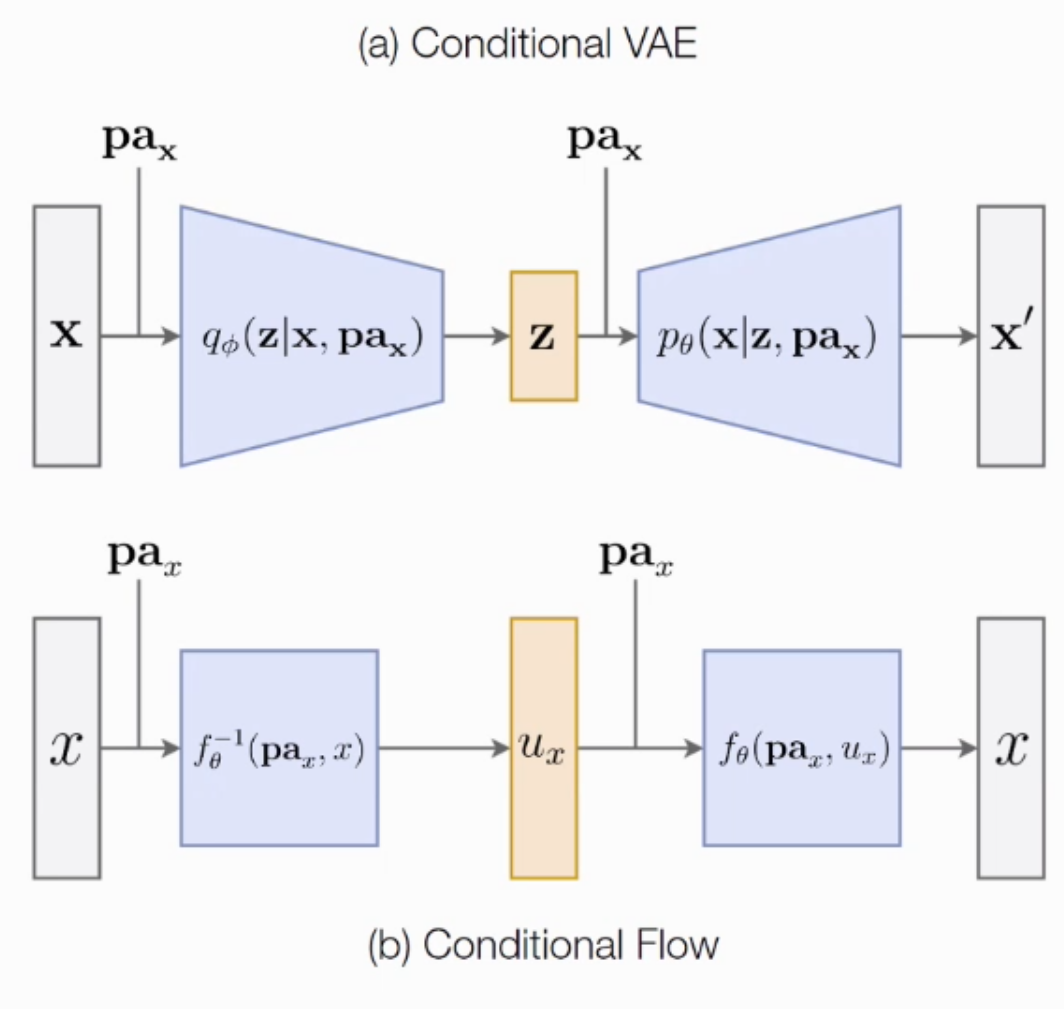
\includegraphics[width=.6\linewidth]{figures/vaes.png}}
    \caption{``conditional vae and the conditional flow look the same. The catch here, is that the attention step is now non-deterministic because the ecnoder produces a distribution of all these encodings and the decoder also produces a distirbution over pixel values.''}
\end{figure}

\begin{figure}[H]
    \centering
    \fbox{\includegraphics[page=34, trim=0cm 0cm 0cm 0cm, clip, width=.95\linewidth]{causality-and-generative-models.pdf}}
    \caption{``We can define the causal mechanism for an image X. The parents of X here are meta infromation like age etc.'' We have g that is decoder model that predicts the per pixel mean and variances. and the H mechanism is how we smaple from this distribution. The encoder is approximately invertible. Therefore, we have a factorizeed exogenous noise decomposition. To calucalte the posterior it is apprxoimated by the encoder mapping and the inversion of the dterministic sampling procedure}
\end{figure}

\begin{figure}[H]
    \centering
    \fbox{\includegraphics[page=35, trim=0cm 0cm 0cm 0cm, clip, width=.95\linewidth]{causality-and-generative-models.pdf}}
    \caption{1) encoding: pass it through encoder and receive z. Then decode. after you invert the sampling in the observation space so given its an image $X$ we subtract the predicted mean and divide by the predicted variabce per pixel. 2) next step is to perform some intervention upsteam. e.g. if we have a causal graph with various dependencies between the parents, if we intervene on one of them and compute the value of the new parents, (the $\tilde{\cdot}$ values) and set these to 0 values. 3) in the final step we pass the new values through the decoder and plug values of epsilon and z  that we abducted in the abduction step as well as the new values of the parents to condition with the decoder. \emph{This applies to, if we want to see what the image would look like if we had a different age.}}
\end{figure}

\begin{figure}[H]
    \centering
    \fbox{\includegraphics[page=36, trim=0cm 0cm 0cm 0cm, clip, width=.95\linewidth]{causality-and-generative-models.pdf}}
    \caption{This is not scalable to high resolutions, so we need a more powerful generative model that is still amenable to principal deduction ut can also scale up to higher resolutions. A natural solution is the heirarchical vae; here we have $L$ latent variables instead of just one.}
\end{figure}

\begin{figure}[H]
    \centering
    \fbox{\includegraphics[page=37, trim=0cm 0cm 0cm 0cm, clip, width=.95\linewidth]{causality-and-generative-models.pdf}}
    \caption{The goal is simliar; optimize model to be close to a given data distribution. The only difference from the VAE objective is that we now have a multitude of latent variables and factorize across the $L$ layers.}
\end{figure}

\begin{figure}[H]
    \centering
    \fbox{\includegraphics[page=38, trim=0cm 0cm 0cm 0cm, clip, width=.95\linewidth]{causality-and-generative-models.pdf}}
    \caption{caption}
\end{figure}

\begin{figure}[H]
    \centering
    \fbox{\includegraphics[page=39, trim=0cm 0cm 0cm 0cm, clip, width=.95\linewidth]{causality-and-generative-models.pdf}}
    \caption{boxed term is MSE loss. point being here is that it is a hierarchcal VAE with a different inference model.}
\end{figure}

\begin{figure}[H]
    \centering
    \fbox{\includegraphics[page=40, trim=0cm 0cm 0cm 0cm, clip, width=.95\linewidth]{causality-and-generative-models.pdf}}
    \caption{``We had to figure out a couple of ways to condition these VAEs. The first, is to retrain the role of the latent variable as being part of the exogenous noise for $X$. in this case, the latent varibales are independent o fhte values of the parents. So when inferring these lantent vairbales they on't get acecso the vlaues of the parents.'}
\end{figure}

\begin{figure}[H]
    \centering
    \fbox{\includegraphics[page=41, trim=0cm 0cm 0cm 0cm, clip, width=.95\linewidth]{causality-and-generative-models.pdf}}
    \caption{The second option is to include a conditional prior, so the latent varibles do see the values of the parents.}
\end{figure}

\begin{figure}[H]
    \centering
    \fbox{\includegraphics[page=42, trim=0cm 0cm 0cm 0cm, clip, width=.95\linewidth]{causality-and-generative-models.pdf}}
    \caption{The way you construct this is by stacking residula blueing blocks into a u-net style architecture. These should then be trained to predict the mean and variabce of the latent variables.}
\end{figure}

\begin{figure}[H]
    \centering
    \fbox{\includegraphics[page=43, trim=0cm 0cm 0cm 0cm, clip, width=.95\linewidth]{causality-and-generative-models.pdf}}
    \caption{using this conditional prior as an implication induces a latent mediateor. These latent varibales are no longer part of the exogenous noise, this is becuase they are caused by things within the model (there is a directed arrow from the parents to the latent variables now). This is still Markovian because the way you give rise to these latent vairblaes still depends on some external independent noise when you sample them.}
\end{figure}

In these diagrams, the grey nodes are observed variables, the middle are exogenous noise u terms and on the right we have unobserved counterfactual values. The key thing is that the exogenous noise is shared between the factual observed and counterfactual branches.

\begin{figure}[H]
    \centering
    \fbox{\includegraphics[page=44, trim=0cm 0cm 0cm 0cm, clip, width=.95\linewidth]{causality-and-generative-models.pdf}}
    \caption{this allows you to apply causal mediation analysis defintion above. the main takeaway, is how the parents affect the image vs how the latent variables affect the image. We can visualise this and understand what our interventions are doing when we're chanign things and confusing counterfactuals.}
\end{figure}

\begin{figure}[H]
    \centering
    \fbox{\includegraphics[page=45, trim=0cm 0cm 0cm 0cm, clip, width=.95\linewidth]{causality-and-generative-models.pdf}}
    \caption{Here we have 4 observed variables and a predefined causal graph. Each column is a different intervention; so we can change the digits, the thickness and the intensity. We can see that when we change the thickness, it obeys the causal graph (thickness causes intensity but the same is not true the other way around).}
\end{figure}

\begin{figure}[H]
    \centering
    \fbox{\includegraphics[page=46, trim=0cm 0cm 0cm 0cm, clip, width=.95\linewidth]{causality-and-generative-models.pdf}}
    \caption{Similar example, we start with a medically assumed causal graph with 6 observed variables. $X$ is one of the variables being the image, we also have ventricle volume, age, brain volume, MRI sqeuencing $M$, sex of patient $S$. Each column here is an intervention on a different attribute. If we change nothing we get a reconstruction back out. Idea here is we're not generating different brains, we generating this particular brain with different attributes.}
\end{figure}

\begin{figure}[H]
    \centering
    \fbox{\includegraphics[page=47, trim=0cm 0cm 0cm 0cm, clip, width=.95\linewidth]{causality-and-generative-models.pdf}}
    \caption{Here we have a different assumed causal graph, but once again it was medically informed.}
\end{figure}

\subsection{Evaluating Counterfactual}

\begin{figure}[H]
    \centering
    \fbox{\includegraphics[page=48, trim=0cm 0cm 0cm 0cm, clip, width=.95\linewidth]{causality-and-generative-models.pdf}}
    \caption{How do we evaluate these counterfactuals? There are a couple theorems above.}
\end{figure}

\subsubsection{Composition Axiom}

\begin{figure}[H]
    \centering
    \fbox{\includegraphics[page=49, trim=0cm 0cm 0cm 0cm, clip, width=.95\linewidth]{causality-and-generative-models.pdf}}
    \caption{Definition above, we can see an example above with high composition; a de-biased model. If we continuously apply the null intervention iteratively and try to reconstruct the image, if the identities are well preserved across tehse iterated applications mechanisms, then we known that the model has high composition. \\
    Conversely, if it has low composition the identity is lost.}
\end{figure}

\subsubsection{Effectiveness Axiom}

\begin{figure}[H]
    \centering
    \fbox{\includegraphics[page=50, trim=0cm 0cm 0cm 0cm, clip, width=.95\linewidth]{causality-and-generative-models.pdf}}
    \caption{Definition above. An example with high effectiveness, if we want to change digit identitiy it will preserve colour, if we want to change colour then it should preserve digit identity. So a model with low effectiveness will be biased.}
\end{figure}

\subsubsection{Reversibility Axiom}

\begin{figure}[H]
    \centering
    \fbox{\includegraphics[page=51, trim=0cm 0cm 0cm 0cm, clip, width=.95\linewidth]{causality-and-generative-models.pdf}}
    \caption{It has to do with cyclic consistency. A model with good reversibility will be able to do this, otherwise it color information will be lost. The reversibility follows from the composition axiom if you use a directed acyclic graph.}
\end{figure}

\begin{figure}[H]
    \centering
    \fbox{\includegraphics[page=52, trim=0cm 0cm 0cm 0cm, clip, width=.95\linewidth]{causality-and-generative-models.pdf}}
    \caption{We identified an inherent trade-off between composition and effectiveness -- when you train counterfactual inference models you want to be good at all of these things, but there seems to be a trade off between composition and effectiveness specifically.}
\end{figure}

\begin{figure}[H]
    \centering
    \fbox{\includegraphics[page=53, trim=0cm 0cm 0cm 0cm, clip, width=.95\linewidth]{causality-and-generative-models.pdf}}
    \caption{caption}
\end{figure}

\begin{figure}[H]
    \centering
    \fbox{\includegraphics[page=54, trim=0cm 0cm 0cm 0cm, clip, width=.95\linewidth]{causality-and-generative-models.pdf}}
    \caption{caption}
\end{figure}

\end{document}